
%% bare_conf.tex
%% V1.3
%% 2007/01/11
%% by Michael Shell
%% See:
%% http://www.michaelshell.org/
%% for current contact information.
%%
%% This is a skeleton file demonstrating the use of IEEEtran.cls
%% (requires IEEEtran.cls version 1.7 or later) with an IEEE conference paper.
%%
%% Support sites:
%% http://www.michaelshell.org/tex/ieeetran/
%% http://www.ctan.org/tex-archive/macros/latex/contrib/IEEEtran/
%% and
%% http://www.ieee.org/

%%*************************************************************************
%% Legal Notice:
%% This code is offered as-is without any warranty either expressed or
%% implied; without even the implied warranty of MERCHANTABILITY or
%% FITNESS FOR A PARTICULAR PURPOSE!
%% User assumes all risk.
%% In no event shall IEEE or any contributor to this code be liable for
%% any damages or losses, including, but not limited to, incidental,
%% consequential, or any other damages, resulting from the use or misuse
%% of any information contained here.
%%
%% All comments are the opinions of their respective authors and are not
%% necessarily endorsed by the IEEE.
%%
%% This work is distributed under the LaTeX Project Public License (LPPL)
%% ( http://www.latex-project.org/ ) version 1.3, and may be freely used,
%% distributed and modified. A copy of the LPPL, version 1.3, is included
%% in the base LaTeX documentation of all distributions of LaTeX released
%% 2003/12/01 or later.
%% Retain all contribution notices and credits.
%% ** Modified files should be clearly indicated as such, including  **
%% ** renaming them and changing author support contact information. **
%%
%% File list of work: IEEEtran.cls, IEEEtran_HOWTO.pdf, bare_adv.tex,
%%                    bare_conf.tex, bare_jrnl.tex, bare_jrnl_compsoc.tex
%%*************************************************************************

% *** Authors should verify (and, if needed, correct) their LaTeX system  ***
% *** with the testflow diagnostic prior to trusting their LaTeX platform ***
% *** with production work. IEEE's font choices can trigger bugs that do  ***
% *** not appear when using other class files.                            ***
% The testflow support page is at:
% http://www.michaelshell.org/tex/testflow/



% Note that the a4paper option is mainly intended so that authors in
% countries using A4 can easily print to A4 and see how their papers will
% look in print - the typesetting of the document will not typically be
% affected with changes in paper size (but the bottom and side margins will).
% Use the testflow package mentioned above to verify correct handling of
% both paper sizes by the user's LaTeX system.
%
% Also note that the "draftcls" or "draftclsnofoot", not "draft", option
% should be used if it is desired that the figures are to be displayed in
% draft mode.
%
\documentclass[conference]{IEEEtran}

\usepackage{url, fancyvrb, framed, multirow, tabularx, graphicx, epstopdf, enumerate, array, cite, algorithmic, fixltx2e}

\usepackage[cmex10]{amsmath}
%\usepackage{breqn}

% correct bad hyphenation here
\hyphenation{op-tical net-works semi-conduc-tor}

\begin{document}
%
% paper title
% can use linebreaks \\ within to get better formatting as desired
\title{NDN Repo: An NDN Persistent Storage Model}


% author names and affiliations
% use a multiple column layout for up to three different
% affiliations
%\author{\IEEEauthorblockN{Michael Shell}
%\IEEEauthorblockA{School of Electrical and\\Computer Engineering\\
%Georgia Institute of Technology\\
%Atlanta, Georgia 30332--0250\\
%Email: http://www.michaelshell.org/contact.html}
%\and
%\IEEEauthorblockN{Homer Simpson}
%\IEEEauthorblockA{Twentieth Century Fox\\
%Springfield, USA\\
%Email: homer@thesimpsons.com}
%\and
%\IEEEauthorblockN{James Kirk\\ and Montgomery Scott}
%\IEEEauthorblockA{Starfleet Academy\\
%San Francisco, California 96678-2391\\
%Telephone: (800) 555--1212\\
%Fax: (888) 555--1212}}

% conference papers do not typically use \thanks and this command
% is locked out in conference mode. If really needed, such as for
% the acknowledgment of grants, issue a \IEEEoverridecommandlockouts
% after \documentclass

% for over three affiliations, or if they all won't fit within the width
% of the page, use this alternative format:
%
%\author{\IEEEauthorblockN{Michael Shell\IEEEauthorrefmark{1},
%Homer Simpson\IEEEauthorrefmark{2},
%James Kirk\IEEEauthorrefmark{3},
%Montgomery Scott\IEEEauthorrefmark{3} and
%Eldon Tyrell\IEEEauthorrefmark{4}}
%\IEEEauthorblockA{\IEEEauthorrefmark{1}School of Electrical and Computer Engineering\\
%Georgia Institute of Technology,
%Atlanta, Georgia 30332--0250\\ Email: see http://www.michaelshell.org/contact.html}
%\IEEEauthorblockA{\IEEEauthorrefmark{2}Twentieth Century Fox, Springfield, USA\\
%Email: homer@thesimpsons.com}
%\IEEEauthorblockA{\IEEEauthorrefmark{3}Starfleet Academy, San Francisco, California 96678-2391\\
%Telephone: (800) 555--1212, Fax: (888) 555--1212}
%\IEEEauthorblockA{\IEEEauthorrefmark{4}Tyrell Inc., 123 Replicant Street, Los Angeles, California 90210--4321}}
\author{\IEEEauthorblockN{Shuo Chen, Weiqi Shi, Junwei Cao}
\IEEEauthorblockA{Research Institute of Information Technology\\
Tsinghua National Laboratory for\\
Information Science and Technology\\
Tsinghua University, Beijing 100084, China\\
chenatu2006@gmail.com}
\and
\IEEEauthorblockN{Alexander Afanasyev, Lixia Zhang}
\IEEEauthorblockA{Computer Science Department\\
University of California, Los Angeles\\
Los Angeles, CA 90095\\
\{afanasev, lixia\}@cs.ucla.edu}}



% use for special paper notices
%\IEEEspecialpapernotice{(Invited Paper)}




% make the title area
\maketitle


\begin{abstract}
%\boldmath
NDN repository (\emph{repo} for short) is a persistent storage model of Named Data Networking, compared with NDN Content Store. NDN makes in-network storage possible because of naming and signature mechanism of network data packets. \emph{NDN repo} is not a built-in part of NDN, but an application conforming to NDN protocol. Application level framing is realized in \emph{repo} design. Network data can be used for application directly.

In this paper, a specification of \emph{NDN repo} is designed to standardize repo operation interfaces. An initial implementation \emph{repo-ng} is presented. Evaluation is conducted compared with \emph{ccnr} of the CCNx project. \emph{Repo-ng} provides more functionalities in remote operation and security policy with reasonable performance tradeoff.

\end{abstract}
% IEEEtran.cls defaults to using nonbold math in the Abstract.
% This preserves the distinction between vectors and scalars. However,
% if the conference you are submitting to favors bold math in the abstract,
% then you can use LaTeX's standard command \boldmath at the very start
% of the abstract to achieve this. Many IEEE journals/conferences frown on
% math in the abstract anyway.

% no keywords




% For peer review papers, you can put extra information on the cover
% page as needed:
% \ifCLASSOPTIONpeerreview
% \begin{center} \bfseries EDICS Category: 3-BBND \end{center}
% \fi
%
% For peerreview papers, this IEEEtran command inserts a page break and
% creates the second title. It will be ignored for other modes.
\IEEEpeerreviewmaketitle

\section{Introduction}

Data distribution is the largest network stream in current Internet. Many web applications like video or image distribution adopts content delivery network (CDN) for quick access of network data. Besides, more and more data are stored in network storage such as Dropbox, Google Drive and Amazon S3. Network and backend storage are commonly separately designed in current TCP/IP network architecture and there is always network packet and storage data presentation transforming process. In this paper, an in-network storage model Named Data Networking repository (\emph{NDN repo}) is proposed based on NDN network. In NDN, network packet is directly identified by the name of the data, not the source or destination identification. Thanks to this mechanism, \emph{NDN repo} directly storages network and application ready data, which realizes the concept of application level framing. \cite{clark1990architectural}

An \emph{NDN repo} is a set of storage application over NDN network managed by single party. It is upon application level without tweaking the NDN protocol. Compared with \emph{Content Store} (\emph{CS}) which provides data packets in-network cache, \emph{NDN repo} provides persistent storage for data objects. The storage of unit is data object and the management scope is based on NDN name prefix. An NDN repo should response interests with managed name prefix with data packets. Besides, NDN repo also offers data object insertion and deletion, fetching data with assigned name prefix and status check of such progresses. An \emph{NDN repo} should conform to the \emph{NDN repo} protocol, which specifies the semantics of NDN packet for repo interaction and basic processes of each functions, such as insertion and deletion. Repo protocol does not limit packet transport control or any security policy.

In this paper, the design of \emph{NDN repo} protocol is demonstrated. The major design goals are: security for remote operation, management and control based on namespace, reliable operation of large data object which can not be framed in a single data packet. Different special cases are detialedly discussed. An initial \emph{NDN repo} implementation \emph{repo-ng} is also demonstrated. It conforms to the protocol and provides interfaces to configure security policy. The boundary of network and storage is broken that data object could be directly used for application and network transportation. Besides, \emph{NDN repo} protocol can be applied for NDN application using data storage service.

The rest of this paper is organized as follows. Section \ref{section-background} introduce the background of \emph{NDN repo}.  Section \ref{section-design} illustrates the design goals of \emph{NDN repo} and how it works. Section \ref{section-implementation} demonstrates the example implementation of \emph{NDN repo} -- \emph{repo-ng}. Section \ref{section-evaluation} evaluates the performance and functionality of \emph{repo-ng}. Section \ref{section-discussion} discusses the evaluation results and tradeoff in \emph{NDN repo} design. Section \ref{section-conclusion} concludes the paper and addresses the future work.

\section{Background} \label{section-background}
\subsection{Named Data Networking}
Named Data Networking (NDN) \cite{zhang2010named} is a data-oriented network architecture which replaces IP with names of data packets as the narrow waist of networking. The essential evolution of NDN is the change of network behaviors from delivering data to a certain destination to fetching data with a given name. \cite{zhang2010named} Because of this change, \emph{interest} and \emph{data object} are imported as network packets for fetching and responding data of given name. \emph{Interest} is the request of network packets containing prefix of names and other constraints. Data packet contains the content of data and the digital signature signed by data producer.

In-network storage means device at network level can not only cache network packet temporarily, but also stores the data packet for local or remote application using directly. NDN makes in-network storage possible because of following reasons: Network packet is identified by source and destination host addresses in IP network, while name of NDN packet is irrelevant with physical endpoints. Any host in NDN network carrying data of given names can response to the \emph{interest}, but hosts besides source and destination cannot retrieve in-network IP packet. Another concern is the privacy of in-network data. Signature in data packet is to resolve authentication and confidentiality of data. \emph{Content Store (CS)} is cache of data packet in NDN router model and it is within network layer.

In \cite{clark1990architectural}, TCP/IP and other layered network architecture are revisited. Data presentation is major cost in network data processing. This presentation process should not be limited to the current network function, but should adjust to certain application wants. Concept of application level framing is proposed to move presentation and transport control from network to application level. This principle is fully adopted in \emph{NDN repo} design.

\subsection{ccnr}

\emph{Ccnr}\footnote{Ccnr: https://www.ccnx.org/releases/latest/doc/technical/RepoProtocol.html} is a subset software of CCNx project\footnote{CCNx: http://www.ccnx.org/what-is-ccn/}. CCN and NDN have the same origin and their designs of architecture are similar. \emph{Cnnr} is a repository that preserving CCN network packet. It supports remote data fetching using interests and local data dump. The functions of \emph{ccnr} is limited. User cannot issue data insertion command remotely and command cannot be verified to apply security policy. This repository protocol is not sufficient for application needs.

\section{Design of NDN Repo protocol} \label{section-design}

\subsection{overall design of repo protocol}

The goal of this section is to demonstrate protocol and discuss concerns on potential failure cases. NDN Repo protocol is specification of NDN network packet and process to operate \emph{NDN repo}. Controls of the network transportation such as flow control, access control and so on are all defined in \emph{repo} application level. To design this \emph{repo} protocol, the following questions must be answered first:

\subsubsection{what is the storage unit}

The basic storage unit is data object. A data object is not just limited to one NDN data packet but defined by application level. The name of data object adopts the naming convention of NDN data packet except that, one data object could be segmented into multiple data packets. Although the data consumer can still access certain segmented packet of a data object, the basic operation unit is advised to be data object. The data object is immutable. If the data producer updates the data object, it should generate the data object of a new version.

Prefix is basic management unit, which means a set of name prefixes are registered to repo and repo will just regulates data objects under such prefixes.

\subsubsection{what functions does the \emph{repo} provide}

For a storage system, the basic operations are \emph{CRUD}. Currently, \emph{repo} offers data object retrieval, insertion, deletion and watch prefix. Data retrieval means \emph{repo} will response interests for data it holds. Data insertion and deletion are put and removal data objects of given names. Watch prefix function means that repo will keep sending interests of given interests for certain time.

\subsubsection{how to identify a repo}

One of the design goal of \emph{repo} is to operate on a designated \emph{repo}. There should be identities to distinguish \emph{repos}. In this design, the identity of \emph{repo} is \emph{repo} name. The format of \emph{repo} name conforms to the URL style of NDN name.

\subsubsection{how to encode command and response}

The command of \emph{repo} function is encoded in \emph{signed interest}\footnote{signed interest: http://redmine.named-data.net/projects/ndn-cxx/wiki/
SignedInterest}. Singed interest is a interest encoded with signature in the component of the name of the interest. This signature is signed by client who issues the command. Once the repo receives the \emph{repo} command, repo can validate the signature and to do specific operation according to the identity of the command. The basic structure of \emph{repo} command is that:

/$\langle repo-name\rangle$/$\langle function\rangle$/$\langle parameter\rangle$/$\langle timestamp\rangle$/
$\langle random-value\rangle$/$\langle SignatureInfo\rangle$/$\langle SignatureValue\rangle$

The last four components are necessary suffix of signed interests. \emph{Repo-name} is the name of the repo. \emph{function} is the name of the function, fox example, \emph{insert} for insert function. \emph{Parameter} is the parameter of the function. Multiple sub-components could be encoded in this parameter name component. For example, the parameter can carry the name of the data inserted for insert function.

Response is the responding data packet for command singed interest. Multiple information could be encoded in the subsection content of the data packet. For example, statuscode can denotes the status for repo to handle the command.

\subsubsection{how to transport command to designated \emph{repo}}

The transport mechanism of NDN is ``pull'', different from ``push'' of TCP/IP. Interest will not be forwarded to a designated host. However, command should be forwarded to the operated \emph{repo}. According to above, each \emph{repo} has its name and the prefix of command interest is \emph{repo-name}. If the \emph{repo-name} is unique and the routing path is generated correctly, the interest would be forwarded to the designated \emph{repo}. If multiple \emph{repos} share the same name, the forwarding results would be influenced by underlying forwarding strategy.

\subsubsection{how to secure the \emph{repo}}

In NDN, data packet carries the signature for validation. \emph{repo} command is encoded in signed interest also carries the signature. Thus, the similar security policy could be adopted to validate the \emph{repo} command. In addition, identity of command issuer is also encoded in the command interest. \emph{repo} can decide whether this identity has the access to the functions. Access control can be made. In \emph{repo} protocol design, policy of trust and access control are not limited. The users can make their own strategies but just conform to the format \emph{repo} commands.

\subsubsection{how to design functions of \emph{repo}}

The design goal or \emph{repo} functions is to make sure the status is visible to the client. This visibility is the basis of process control. For example, function insertion is to put data objects into repo. Client will send the command interest first to ask \emph{repo} to fetch the data with the name in the command parameter. If the client is also data producer, it will wait for the incoming interests. However, client will not know data is successfully put into the \emph{repo}. Client will wait until timeout, and cannot decide what to do. Thus, for each function of \emph{repo}, there should be status check process to status of the process, including whether the data object is successfully put or removed. In \emph{repo} design, different status check command comes with each function. This command will fetch the status and progres during the function operation.

\subsection{Data Retrieval}

As a storage application in NDN, \emph{repo} can provide data objects that it holds. When requester needs to know exactly the target data location, to retrieve a data from \emph{repo}, only data name needs to be specified in interests.  To retrieve a data from \emph{repo}, there is no need for the requesters to know which \emph{repo} owns the data it needs. During \emph{repo} initiation, data request prefixes (which is the data name in most cases) are registered into NDN forwarding daemon (NFD)\footnote{NFD: http://redmine.named-data.net/projects/nfd/wiki}. \emph{Repo} keeps listening to its registered prefixes and only these registered requests will be forwarded by NFD to this \emph{repo}. To guarantee efficiency of data retrieval, only the names of data that \emph{repo} current maintains should be registered. Once the \emph{repo} receives a request, it will response the data if it currently owns, otherwise, it will ignore the request.

\subsection{Data Insertion}

\emph{Repo} data insertion represents the process that inserting a specific data object into \emph{repo}, either obtained from local or remote node in the network. Data insertion is necessary since it is the only mechanism to append new data into \emph{repo}.

Data insertion process starts from receiving a signed interest. Instead of providing the data directly to \emph{repo} (since in most cases, the client who sends the signed interest does not have the target data), the signed interest gives instruction on how to get the data. The signed interest should specify the data name that will be inserted, and \emph{repo} can use these information to request the data in network by sending normal interest.

To insert data efficiently and correctly, \emph{repo} provides three different types of insertion: single insertion, insertion with selectors\footnote{selctor: http://named-data.net/doc/ndn-tlv/interest.html\#selectors} and segmented insertion. The signed interest will give \emph{repo} instruction that which insertion mechanism should be adopted.

\begin{enumerate}
\item Single insertion can be used to fetch the object with small size, which can be encoded into one single data packet. Only one interest can bring back the whole object and \emph{repo} store the data after data arrives.
\item Insertion with selectors will be triggered when signed interest contain name selectors. Selectors are used to narrow down the scope that the name prefix refers to. The normal interest that \emph{repo} sends to fetch the data should contain the exact same selectors specified in singed interest.
\item Segmented insertion deals with large object whose size exceeds the upper bound of one single data packet. \emph{Repo} will send multiple interests with same name prefix but incremental sequence number to fetch the segments of large object. The data fetching interests can be sent in pipeline. To avoid too much data come back, there can be congestion and flow control of sending interests. The implementation of control is not stipulated in protocol but defined by concrete implementation.

    Besides, for segmented insertion, start block id and end block id, which represent the first and last segment \emph{repo} should fetch respectively, can be specified in signed interest. It is possible that start block id and end block id are not specified at the same time. The default start block id is zero, which represents \emph{repo} should fetch from the first existed segment. However, there is no default end block id since the total number of segments for different object varies with the object size. And a problem arises due to \emph{repo} does not have the knowledge about which segment is the last one. If the end block id is not specified, \emph{repo} will continuously fetch the next segments even if they are not existed. There are two methods working together to avoid this problem. 1) The data producer who responds the data can specify the final block id (the last segment number that existed) in every segment data. When \emph{repo} receives the segments with the final block id specified, it will know which sequence number is the last one and when should stop insertion process. 2) \emph{repo} sets up a timer when end block id is not specified. When timeout happens, \emph{repo} will stop fetching data to store and end insert process. If the segment data with the final block id arrives, this timeout timer will be dismissed.
\end{enumerate}

Retransmission mechanism is used to handle data packet loss. The timeout for an interest may infer data packet loss. Whenever timeout happens, \emph{repo} will retransmit the interest. \emph{Repo} will stop the insertion process until the total number of retransmission reach a certain value.

To track the insertion process, a check command is used to get the current \emph{repo} status. The check command is periodically issued by the same client who sends the insertion command. It can bring back a status code which gives the client a hint that whether the insertion is successful.

\subsection{Data Deletion}

To manage data more easily and remove unnecessary data, \emph{repo} supports data deletion. The process of deletion is similar to insertion, starting from receiving deletion signed interests. Instead of sending normal interest to fetch data, during deletion, \emph{repo} only needs to find the data whose name is specified in signed interest and remove it
from local database and index.

Similar to insertion, there are also three types of deletion: single deletion, deletion with selectors and segmented deletion. The process of these deletions are introduced as follow:

\begin{enumerate}
\item Single deletion is used to delete data packets (may not be a single one) stored in \emph{repo}. It will delete all the data objects that satisfy the name specified in signed interest (the name is the prefix of the data name).
\item Deletion with selectors is triggered when signed interest contain name selectors. \emph{repo} will remove all the data that match the selectors. Selector in deletion command is not the same as that of insertion. In this case, selector selects all the data objects that conforms to the constrains of selectors, not just one data object.
\item Segmented deletion is used to delete data objects segmented into multiple data packets. Start block id (optional, default is zero) and end block id (required) can be used to select the segments that should be deleted.
\end{enumerate}

From above, we can see that deletion process removes as much data as possible when receives a signed interest. It can also remove all the data under certain name space by only specifying the name space prefix in signed interest. In this way, \emph{repo} can achieve efficient deletion by issuing minimum number of interests. Besides, there are two methods to remove exact one data packet in \emph{repo}: 1) specify the full name in signed interest (since \emph{repo} use the longest-prefix match algorithm to find data) or 2) set the selectors to locate the exact target data.

There is also a similar check command used to check the status of \emph{repo} deletion. The check command will be sent periodically by the client after a deletion command is issued. This check command will bring back the status code which notifies the client whether the data has been deleted or not.

\subsection{watched prefix}

With the hierarchical name system and selectors mechanism, \emph{repo} can support a new insertion algorithm, watched prefix. Watched prefix allows \emph{repo} to keep watching certain name spaces and insert all the data under that name spaces. Besides, \emph{repo} is no longer limited to insert only existed data by using watched prefix. It can obtain some data that are generated after the moment it receives the command, by periodically watching those data in the network. Normal insertion process cannot support this function since \emph{repo} will try to fetch the data immediately when it receives the signed interest, and insertion will fails if there is no such data in network. For normal insertion, inserting a data is an instant process, but for watched prefix, it is a lasting and continues process.

When \emph{repo} receives the watched prefix signed interest, it will start this process. The signed interest need to specify the prefix that \emph{repo} should watch. \emph{repo} automatically and periodically generates the interests with that prefix and sends them into the network. If there are data returning back, \emph{repo} will update the interests by setting the exclude selector to exclude received data. In this way, \emph{Repo} can avoid receiving duplicated data multiple times. If there is no data returning until timeout, \emph{repo} will resend the same interest.

Besides, watched prefix process can be stopped in three different ways: 1) receive stop command, which is also a signed interest, 2) process timeout or 3) the total number of interests have been sent exceeds a certain value. 1) provides a method to manually terminate this process and both 2) and 3) can be used to stop the process automatically. The check command can also be used in watched prefix process to check whether the process is still running.

Furthermore, there is no limitation for how many prefixes a Repo can watch at the same time. It is entirely possible that a \emph{repo} watches multiple prefix simultaneously. Every watched prefix process can work independently without interference.

\section{implementation of repo -- repo-ng} \label{section-implementation}
\emph{Repo-ng} (NDN repo of new generation) is an implementation of NDN persistent in-network storage conforming to \emph{NDN Repo} protocol. It uses ndn-cxx as NDN client library and database Sqlite3 as underlying data storage.

\subsection{Repo Storage Design}

The design of data packet storage of \emph{repo-ng} consists of index and storage components. Index is sorted associative container for Name stored in memory and storage is consistent storage for read, write and delete of data packet.

Underlying storage offers structured API for retrieval, adding and removal of data packets. Sqlite3 is chosen to be the underlying storage for its well cross-platform, self-contained, serverless, and zero-configuration properties.

Index offers fast query of interest in memory. When an interest comes to \emph{repo}, \emph{repo} will query the index with the name and selector to select the id of data packet which is consistent with that of underlying storage. The structure of each entry index is (Id, Name, KeyLocatorHash). Name is the name of data packet. KeyLocatorHash is the hash of key locator of data packet.

In current \emph{repo-ng} design, the data structure of repo-index is skip list. Although skiplist, Btree and other balanced tree all have O(n) query and insertion complexity, skip list has very low inherent constant-factor overheads. Besides, operations of skiplist are much easier to implement. \cite{pugh1990skip}

\subsection{Tust Model and Access Control}

\subsubsection{Tust Model}

Both signed interest and data can be validated by \emph{repo-ng}. Whether or not validating is an option that can be configured. However, validation of command interest is highly recommended. In \emph{repo-ng} implementation, ``validator-config'' which is part of NDN basic library ``ndn-cxx'' is used as validator. The configuration file follows the format of validconf\footnote{validconf: http://redmine.named-data.net/projects/ndn-cxx/wiki/
CommandValidatorConf}.

\subsubsection{Access Control}
When a command interest is coming, the access control mechanism will apply the rules in Access Control List (ACL) to interest one by one, until find the best-match rule for interest. The matching process uses the longest-prefix match to compare the data prefix, repo-prefix specified in each rule with the data name and repo-name specified in signed interest respectively. Only when the two comparisons satisfy the relationship requirement can the rule be a validated rule.

The design of ACL is referred to the format of validconf. The conceptual ACL is like Table \ref{ACL}.

\begin{table*}[htbp]
\centering
\caption{Access Control List}
\label{ACL}
\begin{tabular}{ | c | c | c | c | c | c | }
    \hline
    repo-prefix & relationship & data-prefix & relationship & write-access & delete access \\ \hline
    /repo/example/1 & Is-Prefix-Of & /data/example/1 & Equal & 1 & 0 \\ \hline
    /repo/example/1 & Equal & /data/example/2 & Is-Prefix-Of & 0 & 1 \\ \hline
    /repo/example/2 & Is-Prefix-Of & /data/example/3 & Is-Prefix-Of & 1 & 1 \\ \hline
\end{tabular}
\end{table*}

Repo-prefix is the repo-prefix in \emph{repo} command interest. Data-prefix is that in RepoCommandParameter. Write and delete access defines the access of insertion and deletion.

\subsection{Transportation Control}
In process of insertion, after \emph{repo} receiving the insertion command for segmented data, it will send multiple interests for data packets. If these interests are sent in a burst, the round trip time will be large for some interests and it is difficult to set interest lifetime. So flow control is necessary.

A basic credit based flow control is implemented for insertion command. There is credit number to count the waiting interest request. Once an interest is sent, the credit minus one and if an interest is satisfied by one data. If credit is equal or less than 0, the \emph{repo} stops sending interests. The original credit number could be adjusted according to the count of interest on the wire.

In addition, if an interest is timeout. The same interest could be retransmitted for certain times that can be configured. The retransmitted interest will not subtract the credit.

\section{Evaluation} \label{section-evaluation}

To fully understand the characteristics and benefits of \emph{repo} storage mechanism, in this section, the performance of \emph{repo} is evaluated. The evaluation can be separated into 3 parts: local and network access on physical machine, transport control of data insertion

Local and network access are testes on physical machines. Hardware platform: HP Z220 work station with 3.4 GHz Intel Core i7 processor of 8 cores, 16GB memory, 2T hard drive with 7200rpm, Ethernet Card 1000Mbps.  Lenovo notebook with 1.74GHz Intel Core i3 processor of 2 cores, 2GB memory, 500G hard drive with 7200rpm, Ethernet Card 1000Mbps.

Simulation-based experiments to evaluate \emph{repo} performance under different conditions. NS3\footnote{ns-3: a discrete-event network simulator for Internet systems:
http://www.nsnam.org} with ndnSim \cite{afanasyev2012ndnsim} model is used to simulate multiple scenarios.

\subsection{local access}
In this part, the performance of \emph{repo} storage system, which includes database and index, is fully evaluated. The speed of data fetching, insertion and deletion of data packets are measured. In addition, comparison between \emph{repo} over NFD platform and \emph{ccnr} over \emph{ccnd} platform are conducted.

\emph{Repo} and \emph{ccnr} both supports retrieving and inserting data packets, but \emph{repo} also supports deleting data packets from repo. In this section, all the operations are tested on one host. The data packets are directly generated in memory to avoid hard drive I/O overhead. Access control is not configured. The following are scenarios of tests:

\begin{enumerate}[a]
\item Put data packets with 1200 bytes of data content into a clean \emph{repo-ng}. Validation is off.
\item Put $10^3$ data packets with and without validation.
\item Retrieve data packets of 1200Bits from \emph{repo-ng}
\item Remove data packets from \emph{repo-ng} which carries data packets of 1200Bits. Validation is off.
\item Rebuild index from database snapshot when \emph{repo} restarts.
\item Put data packets with 1200 bytes of data content into a clean \emph{ccnr}.
\item Retrieve data packets of 1200 bytes from \emph{ccnr}.
\end{enumerate}

Table \ref{local-repo} shows the results of \emph{repo-ng} speed from case a to case e. The unit of result is MBps. ``put -s'' and ``put-s-v'' mean insert commands into a clean \emph{repo-ng} with and without validation

\begin{table*}[htbp]
\centering
\caption{Local Access of Repo-ng}
\label{local-repo}
\begin{tabular}{ | c | c | c | c | c | c | c | c | c | }
    \hline
    packet count & put & get & remove & rebuild & put-s & put-s-v & ccnr-put & ccnr-get \\ \hline
    $10^3$ & 0.692 & 16.881 & 15.584 & 120 & 0.041 & 0.038  & 1.336 & 0.869\\ \hline
    $10^4$ & 0.715 & 16.585 & 25.974 & 153.846 & & & 8.778 & 4.180 \\ \hline
    $10^5$ & 0.719 & 16.634 & 29.843 & 158.521 & & & 24.995 & 13.258 \\ \hline
    $10^6$ & 0.713 & 12.918 & 26.266 & 95.610 & & & 28.323 & 18.266\\ \hline
\end{tabular}
\end{table*}

Table \ref{local-repo} shows the comparison of throughput between \emph{repo-ng} and \emph{ccnr}. The speed of insertion of \emph{ccnr} is far more higher than that of \emph{repo-ng}. One of main reason is the underlying storage of these systems. The storage of \emph{ccnr} is rather simple by appending new content objects in the \emph{ccnr} file. In \emph{repo-ng} design, it would support more complex query (selector) of data packets, so it adopts structured storage database. The process of database insertion is far more complex than just appending a file. The speed of fetching is comparable between \emph{repo-ng} and \emph{ccnr}. The speed of fetching drops a little as the mounts of packet grows. The index of \emph{repo-ng} is based on skiplist. It will took more time when index gets larger. Besides, query of database will get slower when data gets larger.

\subsection{network access}
HP Z220 and the notebook are directly connected. Notebook works as client and repo-ng runs on HP Z220. Case a to case d in local access section are tested as table \ref{network-repo} shows.

\begin{table}[htbp]
\centering
\caption{Network Access of Repo-ng}
\label{network-repo}
\begin{tabular}{ | c | c | c | c | c | c | }
    \hline
    packet count & put & get & remove & put-s & put-s-v \\ \hline
    $10^3$ & 0.396 & 2.230 & 8.053 & 0.033 & 0.032  \\ \hline
    $10^4$ & 0.423 & 3.490 & 21.898 & & \\ \hline
    $10^5$ & 0.0.424 & 3.476 & 24.964 & & \\ \hline
\end{tabular}
\end{table}

Compared with local access, the speed drops due to the network latency between the two hosts. However, there is a great speed drop on retrieving data packets. Different resources of client and \emph{repo} are tested to track down the performance bottleneck. We see that the  load of client CPU usage is up to 70\%. This is caused by the process of inserting data. When inserting data into the \emph{repo}, \emph{repo} will issues multiple interests for each data packet. The possessing of these interests would be a great load for the low hardware setting notebook.

\subsection{Control of Data Insertion}

Basic flow control and retransmission are implemented for data insertion. In this section, proportion of successful data insertion are tested against different link drop rate with or without data retransmission. This retransmission is implemented on application level. The retransmission time is set to 3 in this test. The underlying NDN network does not provide any transportation control. As shown in Fig\ref{drop-rate}, the successful insertion with retransmission is apparently better than that without retransmission. This proves the functionality of control of application level.

\begin{figure}[htbp]
\centering
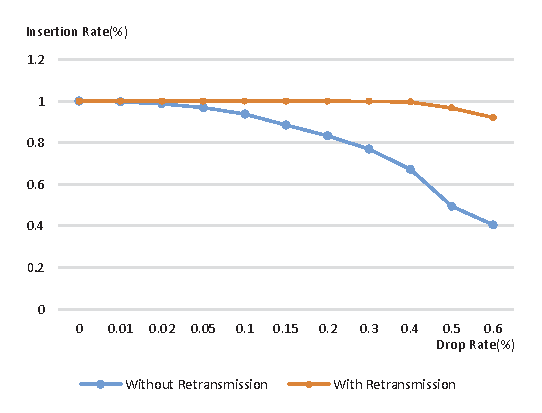
\includegraphics{drop-rate.eps}
\caption{proportion of successful insertion against drop rate}
\label{drop-rate}
\end{figure}

\section{discussion} \label{section-discussion}

In this section, we discuss the advantages and disadvantages of current \emph{repo} design, which would provide an instruct on how \emph{repo} should be used and its current limitation.

\subsection{Advantages}
As an application level storage model, \emph{repo} enjoys many benefits compared with other storage models. We will discuss the benefits in three different aspects: security, scalability and flexibility.

\subsubsection{Security}

By setting up the validator provided by ndn-cxx security library, \emph{repo} can validate any coming signed packets. The validation can make sure the integrity and correctness of data packets. The access control mechanism can protect the privacy of certain data packets by denying the retrieval and any moderation for these data. Both of these two mechanisms are not supported in other storage systems, like \emph{ccnr}.

\subsubsection{Scalability}

As an application level storage system, \emph{repo} can be deployed in any nodes in NDN network. It is proved that multiple \emph{repo} can work fairly in the same network, and the evaluation is not presented due to limited space. Multiple \emph{repos} can also be set up on the same host for different usages.

\subsubsection{Flexibility}

Compared with general network storage systems, \emph{repo} stores application level objects and network ready data packet. Therefore mapping between storage data and network data can be easily avoided, which improves the performance of storage. Besides, \emph{repo} supports remote control which is implemented by signed interests. Clients can issue signed interests to instruct \emph{repo} what should do next, either fetch and insert data from somewhere or delete certain local data. The signed interests can also be broadcasted to all the \emph{repos} in the network, which provide them same actions. It would be very convenient and efficient to globally delete certain malicious data.

\subsection{Disadvantages and Future work}

Although there are many benefits using \emph{repo} to serve as network storage, the existing \emph{repo} design and implementation is incomplete and can be further improved.

Firstly, current \emph{repo} design is single-thread process, which leads to inefficiency of serving multiple client. insertion or removal of a large amount of data packets would block the process and other requests cannot be handled immediately. Secondly, synchronization mechanism is necessary for future design. Although the broadcasted signed interests can be used to provide global instructions, the consistency among multiple \emph{repos} cannot be guaranteed. Besides, the signed interests cannot synchronize the existing data in the \emph{repo}, since the client who issues the signed interest may not have the knowledge about what data repo maintains. In this way, the synchronization mechanism is necessary.

\section{conclusion} \label{section-conclusion}
In this paper, the protocol of \emph{NDN repo} is demonstrated and an implementation of NDN protocol, \emph{repo-ng} is developed. Compared to CCNx Repository Protocols, \emph{NDN repo} supports more functions and provides validation and access control. The design of repo-ng is demonstrated and evaluation shows the efficiency between ccnr and repo-ng. Although repo-ng is less efficient in simple data packets retrieval and insertion, it provides more functions especially remote operations. The concept of application level framing is implemented in the \emph{repo} design. The network data packet can be directly possessed upon application level, which is reasonable design especially for storage system.

\section*{Acknowledgment}
This work was supported in part by National Natural Science Foundation of China (grants No. 61472200 and No. 61233016) and Ministry of Science and Technology of China under National 973 Basic Research Program (grant No. 2013CB228206).

\bibliographystyle{IEEEtran}
\bibliography{IEEEabrv,repo}
% that's all folks
\end{document}


